\chapter{Introduction}
\label{chapter:Introduction}
After over 50 years of miniaturization with the pace of Moore's law\cite{cmcoic}, transistor shrinking is reaching its limits\footnote{A prediction by the 2015 International Technology Roadmap for Semiconductors (ITRS)}, and the increase in CPU-clock speed has halted for a while now. Until quantum computers become a reality, or another hardware technology emerges, computation speed-ups will be achieved by scaling hardware parallelism---for example, current many-core architectures already support tens of thousands of hardware threads.   In contrast to CPU-frequency scaling, which directly resulted in increased performance of the unmodified (sequential) program, unlocking the power of massively-parallel architectures presents significant challenges.   

{\em First}, it requires the programmer to ``think parallel'', for example, to reason about the parallel nature of recurrences (loops) appearing at various nested levels, and then to make the parallelism semantics explicit in the program---ideally by means of parallel-language constructs rather than by unsafe directives such as OpenMP.

{\em Second}, while arguably, programs are (more) naturally expressed by combining parallel constructs at the same level and at various levels in a nest (a.k.a., nested parallelism), many-core architectures have little support for dynamic parallelism and morally exploit only flat parallelism. It follows that ``someone'' has to rewrite the nested-parallel program into a semantically-equivalent one that uses only flat-parallel constructs. Ideally, the compiler is the one that performs this translation (automatically), but unfortunately, current programming-model and compiler technology is far from effectively and reliably supporting real-world applications. It follows that in many cases, it is the programmer who needs to perform this rewriting by hand in addition to applying other (compiler) techniques aimed at optimizing locality of reference, thread divergence, etc. In essence, efficiently porting by hand a complex application to modern hardware often breaks code modularity/maintainability and requires the programmer to have expert knowledge in compiler analysis. Furthermore, the mainstream parallel APIs are rather low-level, and thus very tedious to program with (e.g., OpenCL, CUDA are the ``parallel assembly'' of our time). 

%Firstly, many real-world examples consist of deeply nested compositions of parallel operators, making it difficult for modern hardware to process. In order to cope with it, software needs to be re-written in a way that makes parallelism explicit. This is non-trivial because
%\begin{itemize}
%    \item it requires the programmer to "think" in parallel
%    \item mainstream programming models are very low-level and thus verbose (e.g. OpenCL, CUDA are the "parallel assembly" of our time)
%    \item optimizing parallelism requires users with deep knowledge of compiler optimizations, as it needs to be performed by hand
%\end{itemize}

{\em Third}, to make matters worse, the optimization recipe is often sensitive to the dataset~\cite{FinPar:TACO}, i.e., optimal performance requires several semantically-equivalent code versions, each tailored to the particularities of a class of datasets.   One potential driver in the process of code-version generation is the degree of parallelism that is actually mapped to the hardware. Common wisdom says that outer parallelism is more beneficial (than inner), so in principle, one should exploit as many levels of outer parallelism as there are needed to fully utilize the hardware, and should sequentialize the rest.  This strategy also benefits locality of reference, because sequentializing inner parallelism may enable tiling opportunities. For example:
\begin{itemize}
    \item The common implementation of dense matrix-matrix multiplication utilizes only the outer two levels of parallelism and it sequentializes and tiles the (innermost) dot product operation, which results in a compute-bound performance behaviour.   However, if not enough parallelism is available in the outer levels, then it is necessary to also exploit the dot product parallelism, albeit resulting in memory-bound behavior.
    \item In the case of sparse-matrix vector multiplication, the computation can be carried out in multiple ways: by using row-wise decomposition, column-wise decomposition, or Checkboard decomposition.   The performance of each depends on the distribution and the skewness of the dataset and can lead to other possible trade-offs, such as locality of reference vs. load balancing (thread divergence).
\end{itemize}

%{\em Third}, applications are typically sensitive to the input data and have to deal with irregular-sized arrays, often allowing multiple levels of parallelism to be explored. This introduces the trade-off between what to efficiently sequentialize and what to parallelize. One simple example of this is the matrix-vector dot product, where the computation can be carried out in multiple ways - once by using row-wise decomposition, another by using column-wise decomposition, and a third way by using Checkboard decomposition. The performance of each depends on the distribution and the skewness of the data and can lead to other possible trade-offs, such as locality of reference vs. thread divergence. This often leads to the need for multiple code versions, making use of different optimization strategies, which also raises maintainability problems\cite{FinPar:TACO}.

\newpage
{\em This thesis} explores the space of optimization techniques aimed at efficiently porting to GPGPU hardware\footnote{General-purpose computing on graphics processing units} of a difficult-to-parallelize, real-world application from the financial domain, namely option pricing by means of trinomial trees.   This application is particularly challenging because:
\begin{itemize}
    \item it uses irregular nested parallelism, which is notoriously difficult to map efficiently to hardware, and 
    \item it exhibits thread-divergence on two (orthogonal) levels, which are difficult to optimize at the same time, but leaving either one unoptimized may significantly degrade performance.
\end{itemize}
An interesting finding of this thesis is that the aforementioned \enquote{common wisdom} is only partly correct. It still holds that sequentializing the inner-parallelism in excess (to the ones needed to saturate hardware) is the right thing to do when the divergence is randomly distributed --- even though this method necessarily leaves one level of divergence unoptimized. However, when the distribution of divergence is skewed on both levels, it is better to exploit all parallelism because this allows to optimize all divergence.\medskip\\
%
{\em Finally}, although all discussed optimization techniques have been implemented manually using CUDA programming, we believe that this thesis may provide useful insights into how to integrate such code  transformations in the repertoire of an optimizing compiler.

%{\em This thesis} is concerned with one such irregular application from the financial domain and will introduce the analysis and studies done in order to apply the transformations needed to parallelize it and possibly increase it's performance by using GPGPU\footnote{General-purpose computing on graphics processing units} execution.

\newpage
\section{Problem Statement}
\label{section:problemstatement}
To succeed on the market, financial organizations strive for higher performance in the tools they use on daily basis. Such examples are financial organizations managing investment portfolios with large number of assets, or financial software providers developing applications for pricing and risk management~\footnote{SimCorp is one such organization trying to investigate and attempt to improve the core pricing functionalities in its product, Simcorp Dimension, by using various parallelization techniques to review the implementations of pricing models used by their clients.}. This has led to an increased interest in HPC~\footnote{High performance computing} solutions, efficiently exploiting hardware parallelism. The Hull-White Single-Factor Model is one of the financial models widely used by financial organizations to simulate random changes in interest rates in order to price derivatives. This model can be implemented using trinomial trees~\cite[pg. 444]{ofod}, \cite{uhwirt} - a generic numerical method known for its higher accuracy and stability compared to other popular models used for this purpose (e.g. binomial trees). While this method allows for the precise estimation of option prices, it is extremely expensive computationally, making it an interesting candidate for parallelization. This thesis studies several optimization recipes used to implement the Hull-White Single-Factor Model using trinomial trees, and it also studies how to combine the resulted code versions into one program that offers high performance across all classes of datasets. The main questions this thesis will try to answer are:\\\\
\textbf{What are the performance trade-offs for parallelizing the Hull-White Single-Factor Model on modern massively parallel hardware and which optimization techniques can yield performance benefits?}\\\\
\textbf{Which techniques for parallelism optimization work best for the different data classes and how do we combine all parallel versions into one program that provides high performance on all data sets?}

\newpage
\section{Birds-Eye View of our Approach}
\label{section:solution}
The thesis will begin with the creation of a proof-of-concept sequential implementation of the model. This will be done in accordance to description provided in Options, Futures, and Other Derivatives~\cite{ofod} and will be carried out in C\texttt{++}. Validation will be done only on single callable European zero-coupon bonds, which is the most basic data input to work with. The rationale for studying the financial background of the  algorithm is that it would enable domain-specific optimizations in early design stages.

The algorithm is concerned with the creation of a trinomial tree, with the shape shown on Figure~\ref{fig:intro:tree}. The tree is built in two passes, referred to as forward and backward propagation. Forward propagation represents the construction of a term structure for the underlying asset by progressing one time step at a time. Backward propagation discounts the asset prices to estimate an option payoff at maturity by going back through the tree. The price of the derivative is estimated by the value obtained all the way back at the root. 

As long as optimizations are concerned, the most important properties of the constructed trees are their widths and heights, which are clearly denoted on Figure~\ref{fig:intro:tree}. Both computation steps have a similar structure: the height dimension represents a time series, and is implemented as a sequential loop, because the computation of a certain timestep (level) in the tree depends on the values computed in the previous timestep. However, the computation along the width axis can be performed in parallel, i.e., for a certain timestep, all points at the same level in the tree can be computed with a map operation. 
%
%Furthermore, the computation steps make use of one array whose length equals the height of the tree, and of several arrays whose lengths equal the width of the tree. 
%
It is straightforward to observe that the number of computations performed for a given option depends strongly on both the width and the height of the tree corresponding to that option. This thesis will be concerned with pricing a large number of derivatives (batches) in parallel, as efficiently as possible. Batch pricing exhibits two nested levels of parallelism: one across options, and one on the width dimension of each option tree. Furthermore, this nested parallelism is irregular, because the heights and widths may vary wildly across options. 
%Furthermore it will be interesting to see the impact of trees with irregular widths and heights.

\begin{figure}[H]
	\centering
	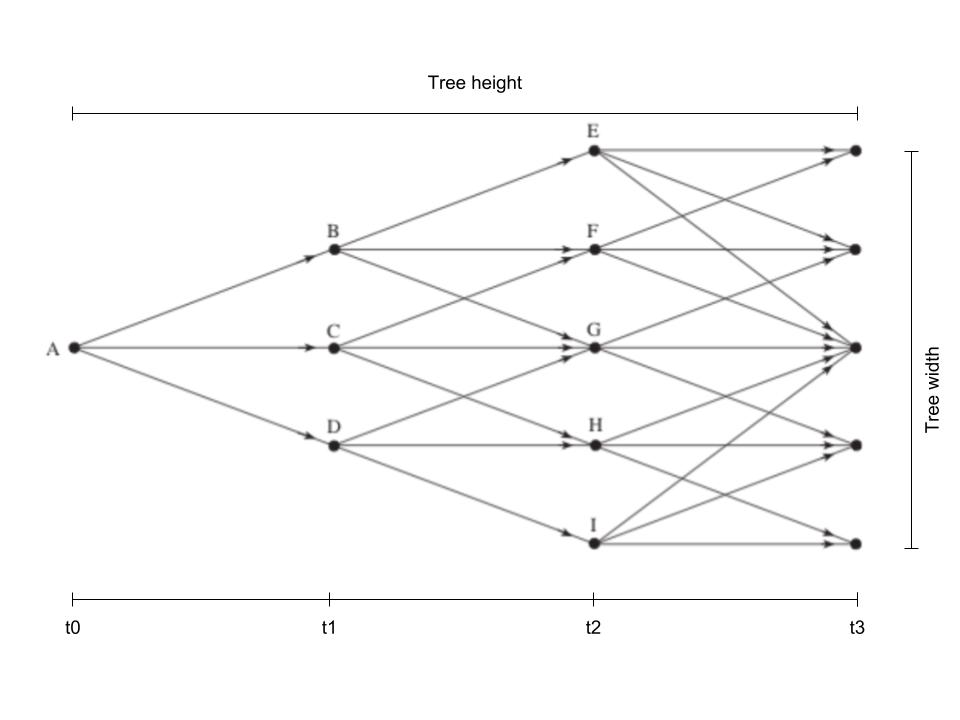
\includegraphics[width=0.8\textwidth]{img/treeconststage1wh.jpg}
	\caption{Example of a trinomial tree constructed for the Hull-White Single-Factor Model, illustrating its width and height.}
	\label{fig:intro:tree}
	\source{Modified by the authors, based on Options, Futures and Other Derivatives\cite[pg. 699]{ofod}.}
\end{figure}

The divergence of widths and heights in a dataset presents several important challenges, but also many optimization opportunities. One of the challenges is to investigate which of the two nested-levels of application parallelism should be mapped to hardware - is it only the outer one or both? 

Exploiting only the outer parallelism is most suited (i) when the batch is large enough to fully utilize hardware parallelism and (ii) when all widths and heights are equal. However, when the heights and widths are highly variant across options, this approach suffers from significant thread-divergence overhead (think load imbalance). It is possible to optimize one of the two divergence factors but not both, for example by sorting the options by their widths (or heights) in a descending order.

The alternative is to exploit both levels of parallelism. This has the advantage that it naturally optimizes the width divergence, while the height divergence can be similarly optimized by sorting.   The problem is that efficient execution requires that the flattening of the two levels of parallelism is performed on bins of options, whose summed widths fit the size of the CUDA block. This is because the flattening transformation introduces many parallel-prefix sums, map, and scatter operations, which would be prohibitively-expensive unless they are performed in fast (scratchpad) memory, which is available only at CUDA-block level. On the other hand, this fast memory, is a very scarce resource. Increasing its footprint may result in decreasing the occupancy of the hardware. In essence this demonstrates an important performance trade-off: optimizing thread divergence may ultimately lead to a decline in hardware occupancy (or locality), i.e., \enquote{there is no free lunch}.

The first parallel approach examined in this thesis refers to the version that exploits only outer parallelism, i.e., it computes a batch of options in parallel, but the pricing of an option is carried out sequentially inside one thread. The challenges for this version are caused by the irregularity of the widths and the heights; they specifically refer to (i) ensuring coalesced accesses to global memory, without wasting too much memory due to padding, and (ii) reducing the thread-divergence overhead by sorting the options based on their widths or heights. The implementations based on this approach have been described in detail in chapters ~\ref{chapter:oneoptionperthread}, ~\ref{chapter:fullflattening} and will be referred to as \textit{CUDA-option} and \textit{Futhark-basic} respectively.

The second parallel approach exploits both levels of parallelism, by packing multiple options and running them in parallel at CUDA-block level. The number of options that can be priced per block depends on their constructed tree widths, whose total sum must not exceed the maximal CUDA block size of 1024. This implies two things: First, this version is not suitable for pricing options with widths larger than 1024, as those cannot be packed into a CUDA block. Second, divergence across the width axis is implicitly optimized by bin-packing options at CUDA-block level. The main difficulty with this implementation is finding the right heuristic for flattening the nested parallelism.  For example, the classical full-flattening approach~\cite{blelloch1994implementation}, while general, is not applicable because it would generate too many arrays located in fast memory, which is a sparse resource. Similar to the previous approach, we can use coalescing, padding and sorting to improve the performance. Exploiting both inner and outer parallelism should help discover performance benefits on some data sets, e.g. the ones which present skewed distributions for both widths and heights. This implementation is covered in detail in chapter~\ref{chapter:multoptionsperthreadblock} and will be referred to as \textit{CUDA-multi}. 

The last parallel approach explores the effects of the classical full flattening~\cite{blelloch1994implementation}. In contrast to the first two versions which have been implemented in CUDA, this version has been flattened out by hand in Futhark~\cite{henriksen2017futhark}, a high-level data-parallel functional language. This approach is similar to the second one, except that all arrays are allocated in slow (global) memory rather than in fast (shared) memory. As such, this version is expected to yield significantly degraded performance in comparison to the remaining two. There is still a narrow niche for it: when the batch size is small and some widths are larger than the block size (then the other two approaches are inefficient or not applicable). However, the real purpose of this implementation is to further emphasize the trade-off between locality of reference and thread divergence: this version is by far the slowest in a large majority of cases, albeit its thread divergence is optimal. This implementation is described in more details in chapter~\ref{chapter:fullflattening} and will be referred to as \textit{Futhark-flat}.
% - sketching the basic solution
% 	- one option per thread
% 	- multiple options per thread block -> difficulty is flattening heuristics the 2 level parallelism in  CUDA block; can further be achieved by bin packing -> by its nature it optimizes the width divergence. 
% 	- a full flattening version achieved in futhark /cite blelock, /cite futhark maybe - implemented in Futhark

%The idea with all implementations is to explore the optimization space by performing both static and dynamic (or hybrid) analysis on the code and the data. Coalescing has proven to be a high impact static optimization on both cuda-option and cuda-multi. Due to the limitations of the Futhark compiler, we have not been able to apply it on the fully-flattened Futhark implementation. Sorting is a dynamic inspector/executor technique which has helped minimize the height/width divergence and shown significant performance improvement.

% - exploring optimization space (static + dynamic or hybrid)
% 	- coalescing (static) is a high impact static optimization on one-option -> state impact
% 	- sorting as inspector executor (dynamic) -> state impact (minimizing height/width divergence) -> in numbers (can be as high as, does not need to be precise)

The thesis will also perform a systematic evaluation of the capabilities of all implementations, by generating and testing them on various datasets that exhibit different distributions of divergence. This will be done in an attempt to study the performance trade-offs on different data and to discover the impact of possible optimization techniques by empirical validation.  

As an empirical evaluation, we will test all implementations on 7 distinct datasets (some of which are random, others skewed). We will show that \textit{CUDA-option} dominates the benchmarks on most datasets (except on the skewed ones), reaching up to \textasciitilde$529\times$ speed-up compared to the sequential implementation. The skewed dataset on the other hand benefits most from \textit{CUDA-multi}, providing up to \textasciitilde$2\times$ speed-up over \textit{CUDA-option}. Furthermore, we will demonstrate that \textit{CUDA-multi} outperforms  \textit{CUDA-option} by up to \textasciitilde$13\times$ for floats and \textasciitilde$11\times$ for doubles when the dataset is small enough. 

% - high-level conclusion 
% 	- one option - in principle we can fix only one of them
% 	- multi - going to sort after heights, because width divergence is already optimized
% 	- empirical evaluation - tested this on N datasets, some are random, some are skewed and it looks that bla bla (this version is better than the other one in this situaiton, and/or bla bla


% - give the high level of A solution - say what is new about our stuff compared to the related work. batch trinom-pricing is challenging due to two levels of divergence (width and height). can show the figure and briefly explain it with the tree, where width and height are shown. briefly and at high level sketch the solution in understandable terms - give the main components e.g. several versions that "make sense"; we are going to demonstrate that there is not a clear winner between them; how to choose the right version?; static analysis? - looking at the code and giving a solution; dynamic analysis? - not looking at the code; hybrid analysis? - combination of the two. analytical measure of the overhead over to divergence and on this we will choose the right version at runtime. done by inspector/executor technique. These things can generally be extracted and done automatically by a compiler in order to solve related problems.

\newpage
\section{Motivation and Relation to Related Work}
\label{section:briefsurveyofrelatedsolutions}

This section briefly surveys related work with the goal of motivating the practical and scientific contributions of this thesis. A more detailed review can be found in Chapter~\ref{chapter:relatedwork}.
%
A rich body of scientific work has studied how to accelerate real-world, computing-starved applications by porting them to GPGPU hardware. Related solutions span several research directions: (i) building native GPGPU libraries, (ii) designing data-parallel languages and (iii) devising compiler transformations aimed at optimizing parallelism.

{\bf Many native GPGPU libraries} have been already developed to support high-performance execution of commonly-used algorithms. Such examples are cuBLAS and cuDNN~\cite{cudnn} that port linear-algebra and deep-learning algorithms, respectively, and a more recent effort of Mathworks and Nvidia that is aimed at accelerating Matlab libraries on Nvidia hardware. Similarly, in the financial domain, efforts have been aimed at accelerating risk modelling~\cite{FinPar:TACO} and derivative pricing~\cite{LexiFiPricing} using Monte-Carlo simulations. We argue that this thesis is of practical interest because, to our knowledge, there is no publicly-available GPGPU implementation of (batched) trinomial pricing. 

{\bf The design of data-parallel hardware-independent languages} have been a heavily scrutinized research topic. In this sense, many domain-specific languages (DSL) have been developed for accelerating image-processing pipelines~\cite{Halide}, iterative stencils~\cite{tang2011pochoir}, data analytics~\cite{HPAT}, deep-learning and mesh computations~\cite{OP2-Mesh,DeliteDSLs}, or specific host-language constructs~\cite{Accelerate-ICFP,StreamJava8,svensson2011obsidian}. However, such DSLs do not typically support nested-composition of parallel constructs, which is the case of trinomial pricing. Finally, even though several data-parallel languages provide some support for nested parallelism~\cite{blelloch1994implementation,henriksen2017futhark}, they are not capable of expressing or deriving (at least) one of the two efficient implementations of trinomial pricing, which are the subject of this thesis.   

%A common pattern can be observed - none the above mentioned methods/compilers can support the building of trinomial trees, due to the irregular parallelism that is required by it. While they are used to transform regular arrays, more complex applications such as the Hull-White Single-Factor Model present other difficulties if higher performance is expected. E.g. it is not possible to implement an effective multiple options per thread block implementation in Futhark, simply because of the the memory allocation constraints in the language. 

\newpage
\paragraph{Relation with compiler analysis.} In this thesis we identify the important performance trade-offs for our application and solve them by hand, taking inspiration from related static and (more) dynamic analyses.  As examples of applications of static analysis, we have optimized spacial locality (i.e., ensured memory coalescing) by working with arrays in transposed form~\cite{LexiFiPricing} and we have performed loop fusion~\cite{PolyhedralOpt} to decrease the number of accesses to global memory. In the implementation of the code version that computes multiple options in one CUDA block, we have drawn inspiration from loop distribution~\cite{PolyhedralOpt} and Blelloch's flattening transformation~\cite{blelloch1994implementation}. This was necessary in order to rewrite the algorithmic specification, which exhibits two-level irregular parallelism, into a composition of flat-parallel constructs.  
%
As example of (more) dynamic analyses, we have used inspector-executor techniques~\cite{Strout:DataItReord,SummaryMonot} to permute the order of the options in a way that minimizes the thread-divergence overhead, and we argue that a similar lightweight inspector can be used to derive a simple predicate that predicts the most suited version of the code for the current dataset.
%
Finally, we argue that the manually-applied optimizations presented in this thesis (i) are likely applicable to other programs, and (ii) they provide useful insights into engineering the compiler infrastructure that would automate the optimization process.


\newpage
\section{Thesis Contributions}
\label{section:thesiscontributions}
\paragraph{Scientific contributions:}
The main scientific contributions of this thesis are:
\begin{itemize}
    \item Research on how the Hull-White Single-Factor Model works in practice and why it is useful
    \item Analysis of how the algorithm behind the Hull-White Single-Factor Model can be flattened to expose more parallelism
    % \item multiple parallel implementations of the Hull-White Single-Factor Model in CUDA
    % \item one fully-flattened parallel implementation of the Hull-White Single-Factor Model in Futhark
    % \item a well-structured project on GitHub containing all implementations with build instructions for each
    % \item data generator for testing edge cases and interesting data distributions
    \item Empirical validation that validates our claims and is supported by tables and plots
    \item Static and dynamic inspector/executor analysis of the model for performance optimization 
\end{itemize}

\paragraph{Practical contributions:}
The main practical contributions of this thesis are:
\begin{itemize}
    % \item research on how the Hull-White Single-Factor Model works in practise and why it is useful
    % \item analysis on how the Hull-White Single-Factor Model can be flattened
    \item Multiple parallel implementations of the Hull-White Single-Factor Model in CUDA
    \item A one-option-per-thread parallel implementation of the Hull-White Single-Factor Model in Futhark
    \item A fully-flattened parallel implementation of the Hull-White Single-Factor Model in Futhark
    \item A well-structured project on GitHub containing all implementations with build instructions for each
    \item Data generator for testing edge cases and relevant data distributions
    % \item empirical validation that validates our claims and is supported by plots
    % \item static and dynamic inspector/executor analysis on the model for performance optimization 
\end{itemize}
	
	
% \section{Road map}
% \label{section:roadmap}
% - road map (only if the thesis ends to be too long)


